\begin{figure}
    \centering
    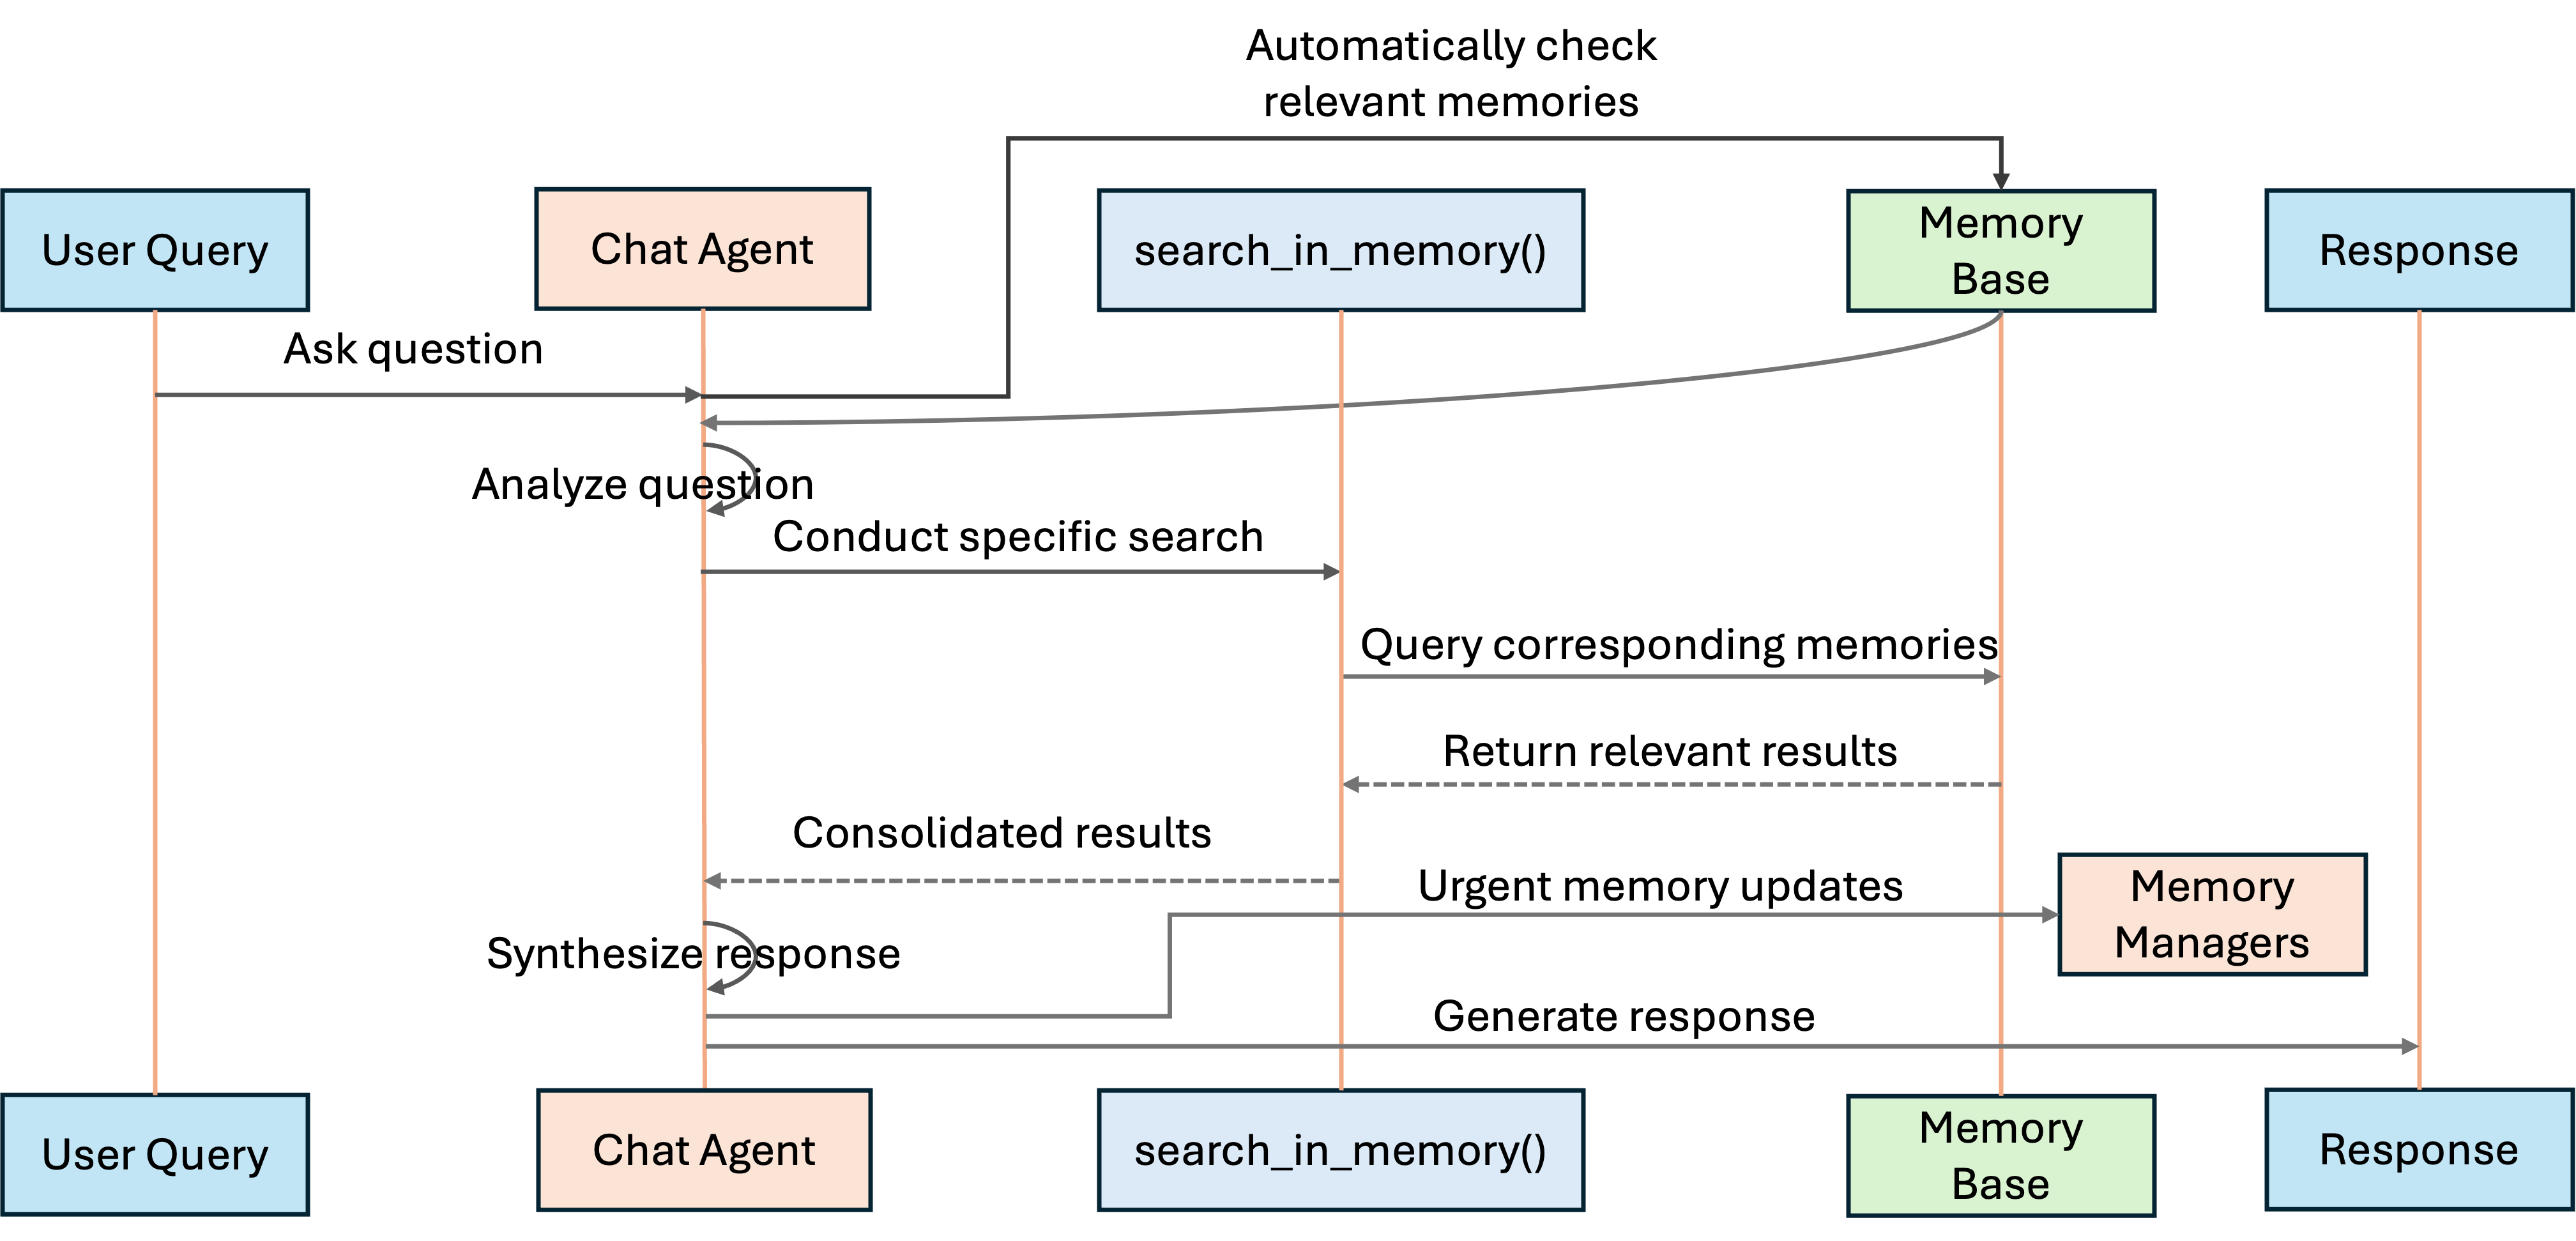
\includegraphics[width=\linewidth]{figures/query_workflow.png}
    \caption{The Workflow of Responding to the User's Query.}
    \label{fig:memory_update_workflow}
\end{figure}

\section{Experiments}

\subsection{Experimental Setup}

\subsubsection{Datasets}
\paragraph{ScreenshotVQA}
We collect a new dataset that contains three PhD students' activities. We created a script that takes a screenshot every second. If the image taken this second is too similar to the last one (similarity $>$ 0.99) then we skip the current image. With this script, three PhD students majored in Computer Science and Physics run the program from a week to a month. The first student is a heavy computer user, which leads to 5,886 images in one day (03/09/2025). The second student uses the computer slightly lighter, leading to 18,178 images for 20 days (05/16/2025-06/06/2025). The third student is the lightest computer user, having 5349 images for over a month (05/02/2025-06/14/2025). Then, with these screenshots, we ask each student to manually create some questions and then we double-check the questions to make sure they are answerable. Eventually, we have 11 questions from the first user, 21 questions from the second user, and 55 questions from the third user. 

\paragraph{LOCOMO} Following Mem0~\citep{mem0}, we choose LOCOMO dataset for a vertical comparison between \ours and existing memory systems. LOCOMO has 10 conversations, where each conversation has 600 dialogues and 26000 tokens on average. There are averagely 200 questions for each conversation, which is suitable for the evaluation for memory systems where we are reuiqred to inject the conversation into the memory and then answer the 200 questions according to the obtained memory. The questions can be classified into multiple categories: single-hop, multi-hop, temporal and open-domain. The dataset also has another category called "adversarial", which is used to test whether the system can identify unanswerable questions. Following Mem0~\citep{mem0}, we exclude this category in our setting to provide fair comparisons with the earlier methods. 


\subsubsection{Evaluation Metrics and Implementation Details}
\paragraph{Evaluation Metrics}
In this paper, for both of the above datasets, we mainly consider the metric \textbf{LLM-as-a-Judge}. Specifically, we use \texttt{GPT-4.1} as the judge to look at the question, answer, and response to predict whether the response addresses the question successfully. 

\paragraph{Implementation Details for ScreenshotVQA}
Across all experiments, we use the \texttt{gemini-2.5-flash-preview-04-17} model as the backbone. We selected Gemini because it integrates seamlessly with Google Cloud, enabling asynchronous image uploads and retrieval. This significantly accelerates processing, as each step requires multiple function calls: one to the meta memory manager and between zero and six to the other memory managers.

\paragraph{Implementation Details for LOCOMO} 
For \ours, since every agent needs to call many functions to successfully insert the information into the memory systems, it requires the language model to have strong abilities on function calling. To this end, we use \texttt{gpt-4.1-mini} as our backbone model as it shows a stronger ability than \texttt{gpt-4o-mini} in terms of function calling. This is also revealled in Berkeley Function Calling Benchmark~\citep{berkeley-function-calling-leaderboard} where \texttt{gpt-4o-mini} has multi-turn overall acc as 22.12, vs the acc of \texttt{gpt-4.1-mini} being 29.75. For LOCOMO dataset, we run the baselines LangMem, RAG-500, Mem0 using the code provided in Mem0~\footnote{\url{https://github.com/mem0ai/mem0/tree/main/evaluation}} with setting \texttt{MODEL} in the \texttt{.env} file as \texttt{gpt-4.1-mini}. Then for Zep, we use the code from their official repo\footnote{\url{https://github.com/getzep/zep-papers?ref=www.getzep.com/blog}} and replace the backbone model with \texttt{gpt-4.1-mini}. For all the baselines, we run their code once, while for \ours and Full-Context method, we run three times to report the average scores. We provide the results of each single run in Appendix \ref{sec:full_experimental_results}. 
The complete code for our evaluation and the predicted results from various baselines and \ours are provided in the \texttt{public\_evaluation} branch\footnote{\url{https://github.com/Mirix-AI/MIRIX/tree/public_evaluation}} in our official repository.







\subsection{Experimental Results on ScreenshotVQA}
For \textbf{ScreenshotVQA}, since existing memory systems such as Letta, Mem0 still lack the ability to process multimodal input, we omit the comparisons with them. We consider the following baselines: 

\textbf{Gemini}. As a long-context baseline, Gemini directly ingests the full set of screenshots to answer the questions. Because the original high-resolution screenshots exceed the model’s context window, we resize them to 256×256 pixels, enabling approximately 3,600 images to fit into a single prompt. We then include the most recent 3,600 images in the prompt and query the model for an answer. Specifically, we use the \texttt{gemini-2.5-flash-preview-04-17} model.

\textbf{SigLIP}. SigLIP serves as a retrieval-augmented baseline. We first use SigLIP to identify the top 50 most relevant images for each query and then prompt Gemini to generate the answer based on these retrieved images. In this setup, we employ \texttt{google/siglip-so400m-patch14-384} as the retriever and \texttt{gemini-2.5-flash-preview-04-17} as the language model.

We evaluate all methods using two metrics: (1) \textbf{Accuracy}, measured via an LLM-as-a-Judge approach comparing the generated responses to ground-truth answers and reporting the average accuracy across the three participants; and (2) \textbf{Storage}, defined as follows—For Gemini, we report the total size of the images after resizing to 256×256. For SigLIP, we report the total size of the original retrieved images in their native 2K–4K resolution. For \ours, we use \texttt{sqlite} as the storage backend and report the size of the \texttt{sqlite.db} file containing all extracted information.

The results are summarized in Table~\ref{tab:screenshotvqa_results}. As shown, \ours significantly outperforms all existing baselines while requiring substantially less storage. Specifically, because SigLIP retains the full set of high-resolution images, its storage footprint is very large, corresponding to the total size of all images in their original 2K–4K resolution. The long-context baseline (Gemini) reduces this by resizing images to 256×256 pixels, but still incurs considerable storage overhead. In contrast, \ours avoids storing raw images altogether and instead maintains only the compact \texttt{sqlite} database of extracted information, resulting in a much smaller storage size. Compared to retrieval-augmented generation (RAG) baselines, MIRIX achieves a 35\% improvement in accuracy while reducing storage requirements by 99.9\%. Relative to the long-context Gemini baseline, MIRIX yields a 410\% improvement in accuracy with a 93.3\% reduction in storage. 

\begin{table*}[]
    \centering
    \resizebox{\textwidth}{!}{
    \begin{tabular}{c|cc|cc|cc|cc}
    \toprule
        & \multicolumn{2}{c}{Student 1} &  \multicolumn{2}{c}{Student 2} &  \multicolumn{2}{c}{Student 3} & \multicolumn{2}{c}{Overall} \\
         & Acc $\uparrow$ & Storage$\downarrow$ & Acc $\uparrow$ & Storage$\downarrow$ & Acc $\uparrow$ & Storage$\downarrow$ & Acc $\uparrow$ & Storage$\downarrow$  \\
         \midrule
        Gemini & 0.0000 & 142.10MB & 0.0952 & 438.86MB & 0.2545 & 129.14MB & 0.1166 & 236.70MB \\
        SigLIP@50 & 0.3636 & 22.55GB & 0.4138 & 19.88GB & 0.5455 & 2.82GB & 0.4410 & 15.07GB \\
        \ours & \textbf{0.5455} & \textbf{20.57MB} & \textbf{0.5667} & \textbf{19.83MB} & \textbf{0.6727} & \textbf{7.28MB} & \textbf{0.5950} & \textbf{15.89MB} \\
        \bottomrule
    \end{tabular}}
    \caption{Experimental Results on ScreenshotVQA.}
    \label{tab:screenshotvqa_results}
\end{table*}



\begin{table*}[!t]
\centering
% \resizebox{\linewidth}{!}{%
\begin{tabular}{p{0.5cm}l|cccc|c}   % ← added a 1.5 cm column on the left
\toprule
& \textbf{Method} & \textbf{Single Hop} & \textbf{Multi-Hop} & \textbf{Open Domain} & \textbf{Temporal} & \textbf{Overall} \\
\midrule
\multirow{7}{*}{\rotatebox[origin=c]{90}{\textbf{gpt-4o-mini}}}
  & A-Mem      & 39.79 & 18.85 & 54.05 & 49.91 & 48.38 \\
& LangMem     & 62.23 & 47.92 & 71.12 & 23.43 & 58.10 \\
& OpenAI      & 63.79 & 42.92 & 62.29 & 21.71 & 52.90 \\
& Mem0        & 67.13 & 51.15 & 72.93 & 55.51 & 66.88 \\
& Mem0$^g$       & 65.71 & 47.19 & \textbf{75.71} & 58.13 & 68.44 \\
& Memobase    & 63.83 & 52.08 & 71.82 & 80.37 & 70.91 \\
& Zep         & 74.11 & 66.04 & 67.71 & 79.76 & 75.14\\
% \cmidrule{2-7}
% & Full-Context & 80.14 & 46.89 & 58.33 & 90.49 & 77.51 \\
\midrule
\multirow{6}{*}{\rotatebox[origin=c]{90}{\textbf{gpt-4.1-mini}}}
 % & Zep & 48.23 & 17.76 & 39.58 & 62.43 & 49.09 \\
& LangMem & 74.47 & 61.06 & 67.71 & 86.92 & 78.05 \\
& RAG-500 & 37.94 & 37.69 & 48.96 & 61.83 & 51.62 \\
& Zep & 79.43 & 69.16 & 73.96 & 83.33 & 79.09 \\
& Mem0    & 62.41 & 57.32 & 44.79 & 66.47 & 62.47 \\
\cmidrule{2-7}
& \textbf{\ours} & \textbf{85.11} & \textbf{83.70} & 65.62 & \textbf{88.39} & \textbf{85.38} \\
\cmidrule{2-7}
& Full-Context & 88.53 & 77.70 & 71.88 & 92.70 & 87.52 \\
\bottomrule
\end{tabular}%}
\caption{LLM-as-a-Judge scores (\%, higher is better) for each question type in the \texttt{LOCOMO} dataset. As mentioned in Mem0~\citep{mem0}, as the average length in this dataset is only 9k, Full-Context is essentially the upper-bound. Thus recovering the performance of Full-Context shows the advancements of \ours. }
\label{tab:locomo}
\end{table*}


\subsection{Experimental Results on LOCOMO}
We compare \ours against the following baselines:

\textbf{A-Mem~\citep{amem}:} A memory system that builds Zettelkasten-style knowledge graphs from user-agent interactions, dynamically linking notes using embedding similarity and LLM reasoning.

\textbf{LangMem\footnote{\url{https://github.com/langchain-ai/langmem}}:} LangChain’s long-term memory module that extracts and stores salient facts from conversations for later retrieval through retrievers like FAISS or Chroma.

\textbf{Zep~\citep{zep}:} A commercial memory API that constructs a temporal knowledge graph (Graphiti) over user conversations and metadata, designed for fast semantic querying.

\textbf{Mem0~\citep{mem0}:} An open-source memory system that incrementally compresses and stores memory facts using LLM-based summarization, with an optional graph memory extension.

\textbf{Memobase\footnote{\url{https://github.com/memodb-io/memobase}}:} A profile-based memory module that tracks persistent user attributes and preferences to enable long-term personalization.

All baselines are re-implemented using the same backbone model (\texttt{gpt-4.1-mini}). We also report the results shown in Mem0~\citep{mem0} where the backbone model is \texttt{gpt-4o-mini}. The results are shown in Table~\ref{tab:locomo}. From the table, we observe the following:

\textbf{Overall:} \ours achieves the highest average J score, outperforming all baselines by a significant margin. It improves upon the strongest open-source competitor, LangMem, by over 8 points.

\textbf{Single-Hop and Temporal:} On fact lookup and temporal-ordering tasks, \ours shows significantly better performances than baselines, which validates the effectiveness of our hierarchical memory storage. 
We note that there is a minor gap between \ours and the Full-Context baseline on Single-Hop questions. Upon reviewing the results, we identified a major reason for this. In some cases, the questions are ambiguous. For example, consider the question \emph{``When is Melanie planning on going camping?''} In the conversation history, Melanie stated \emph{``We’re thinking about going camping next month''} in May, which would suggest \emph{June} as the answer. However, she later mentioned in October, \emph{``Absolutely! It really helps me reset and recharge. I love camping trips with my fam, ’cause nature brings such peace and serenity,''} referring to a more recent trip. Because \ours saves the consolidated event \emph{``On 19 October 2023, Melanie and her family went camping after their road trip,''} it tends to prioritize the confirmed occurrence over the earlier plan, leading to discrepancies when the question expects the planned date rather than the actual event. Other similar ambiguities contribute to the slightly lower performance of \ours on Single-Hop questions.


\textbf{Multi-Hop:} \ours demonstrates the largest gains in this category, outperforming all baselines by over 24 points. For example, in questions such as \emph{“Where did Caroline move from 4 years ago?”}, where the correct answer is Sweden, the supporting evidence is dispersed across multiple parts of the conversation. One part may state \emph{“Caroline moved from her hometown 4 years ago”}, while an earlier statement establishes that \emph{“Caroline’s hometown is Sweden”}. For multi-hop questions like these, \ours achieves better performance because it explicitly stores the consolidated event \emph{“Caroline moved from her hometown, Sweden, 4 years ago”}, removing the need to stitch together partial information at query time. In contrast, full-context methods must first retrieve the partial answer \emph{“hometown”} and then figure out separately that \emph{“hometown”}  refers to \emph{“Swedon”}. These multi-hop questions might be easy for reasoning models like OpenAI-O3, but for non-reasoning models such as \texttt{gpt-4.1-mini}, this additional reasoning step might fail, leading to slightly inferior performance compared with \ours.

\textbf{Open-Domain:} While \ours performs well, the margin between ours and the baselines is narrower. This category of questions usually asks the agent ``what if'' questions, requiring the agent to infer across longer terms. The gap between \ours and Full-Context method show the inherent limitation of RAG methods, which is the lack of global understanding. While \ours is no longer simple RAG, we still rely on RAG to retrieve important information in the memory, which might lead to the bottleneck of our agent in this category.



In summary, these results demonstrate that \ours delivers state-of-the-art performance on LOCOMO while remaining highly efficient and modular. Its component-specific memory management and intelligent routing are particularly effective for long-range multi-hop reasoning.













